\documentclass[main.tex]{subfiles}

\begin{document}

\chapter{The SD-433 Energy spectrum}
\label{chapter:SD433_Spectrum}
\label{chap:sdpectrum}
\selectlanguage{english}

With the developed energy reconstruction from the previous chapter and the proper determination of the full efficiency to have a proper estimation of the exposure, this chapter focuses on the measurement of the cosmic ray spectrum with the \sd{433}.
For this, \cref{sec:raw_spectrum} is devoted to the construction of the raw spectrum. 
After this, the forward-folding formalism is presented in order to fit the spectrum and properly measure the second knee in the cosmic ray spectrum.
Several checks were developed to assess the robustnes of the method and to understand the impact of the different detector characteristics.
In \cref{sec:unfolded_spectrum}, the unfolded spectrum is shown and the robustness of the measurement of the second knee is studied.
Finally, in ~\cref{sec:systematics} the impact of the different sources of systematics is assessed to give a complete picture of the measuerment of the spectrum and the second knee.

%%%%%%%%%%%%%%%%%%%%%%%%%%%%%%%%%%%%%%%%%%%%%%%%%%%%%%%%%%%%%%%%%%%%%%%%%%%
\section{Raw spectrum}
\label{sec:raw_spectrum}
%%%%%%%%%%%%%%%%%%%%%%%%%%%%%%%%%%%%%%%%%%%%%%%%%%%%%%%%%%%%%%%%%%%%%%%%%%%
The energy spectrum describes the differential flux of cosmic rays as a function of their energy.
It is estimated from the number of events recorded in a given energy interval, normalized by the exposure of the detector and the width of the interval.
For the \sd{433}, the dataset described in \cref{chap:sd433_dataset} contains \SDFourThreeThreeNEvents events that pass the 6T5 fiducial trigger with zenith angle lower than $40^\circ$.
These events were recorded between 1 July 2018 and 21 December 2021 above the full-efficiency threshold.

The raw flux in reconstructed-energy bin $i$ is estimated as
\begin{align}
    J_i^{\mathrm{raw}}
    =
    \frac{N_i}{\exposuresym\,\Delta E_i},
    \label{eq:raw_flux}
\end{align}
where $N_i$ is the number of events in the bin, $\Delta E_i$ is the bin width, and $\exposuresym$ is the accumulated exposure.
As determined in \cref{sec:exposure}, the exposure is \SDFourThreeThreeExposure$\pm0.09$ and is energy independent above the full-efficiency threshold.
A logarithmic bin width of $\Delta\lg(E/\mathrm{eV})=0.1$ is used up to $\lg(E/\mathrm{eV})=18.1$, chosen to be compatible with the energy resolution described in \cref{sec:res_and_bias}.
Above this energy, the bin width is increased to $\Delta\lg(E/\mathrm{eV})=0.3$ to increase the number of events per bin and reduce the statistical uncertainties.
The spectrum is referred to as raw because no correction has yet been applied for event migrations between energy bins caused by the finite resolution and bias of the detector.

The left panel of \cref{fig:raw_spectrum} shows the raw flux together with the $68\%$ Poisson confidence intervals.
The number of events in each bin is indicated next to each data point.
Since the cosmic-ray flux decreases approximately as $E^{-3}$, the same measurements are shown multiplied by $E^3$ in the right panel.
This representation reduces the dominant power-law dependence and makes changes in the spectral slope more visible.
A steepening around $\lg(E/\mathrm{eV})\simeq17.3$ suggests the presence of a feature compatible with the second knee, although the detector response must be taken into account before it can be properly measured.

\begin{figure}
    \centering
    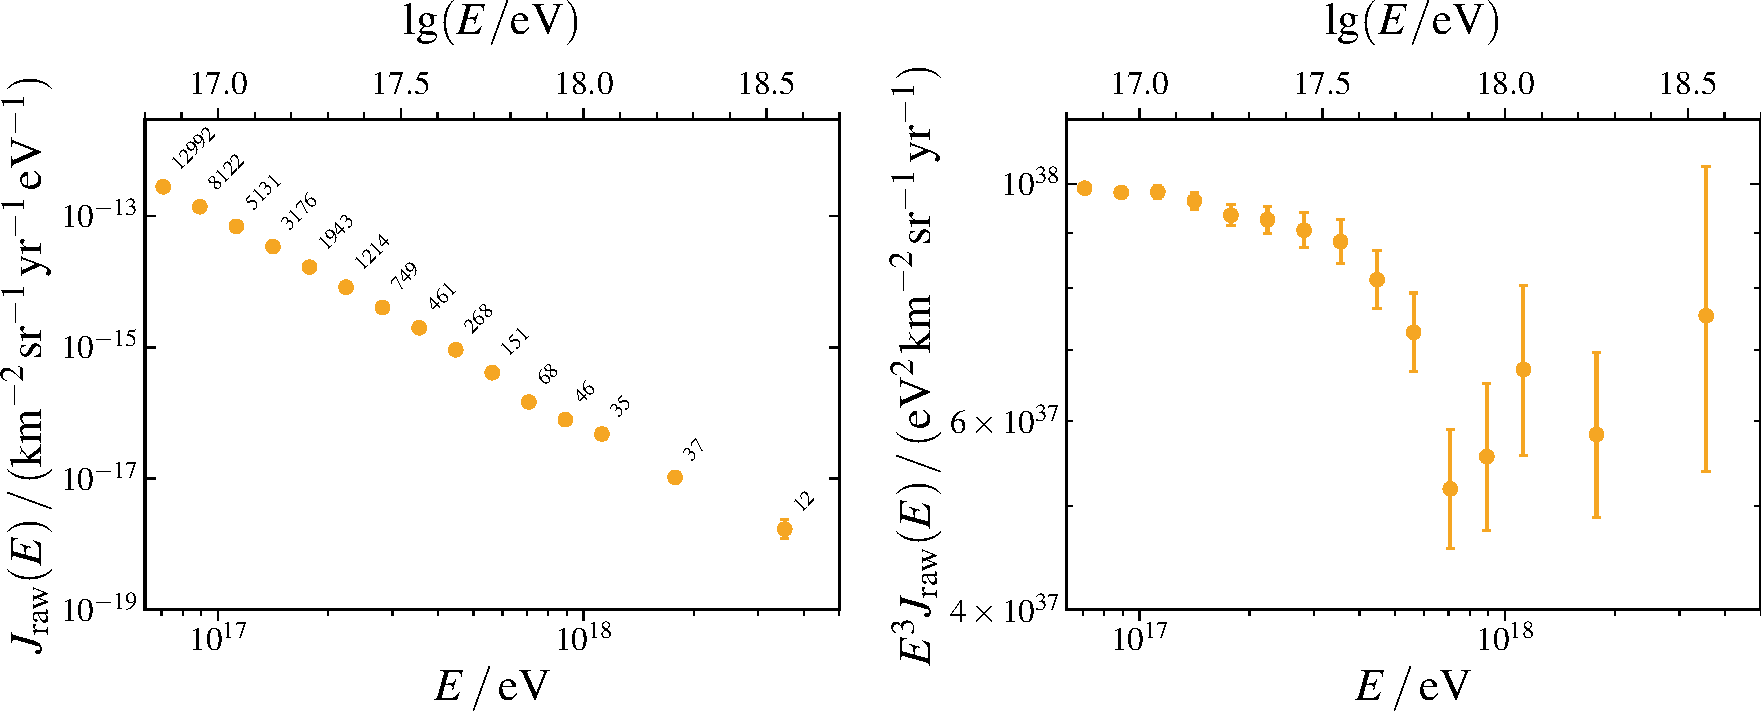
\includegraphics[width=\linewidth]{figures/chapter_spectrum/sd433_raw_spectrum.pdf}
    \caption{
        Raw cosmic-ray spectrum measured with the \sd{433}. The error bars represent the $68\%$ Poisson confidence intervals.
        Left: differential flux as a function of reconstructed energy; the numbers indicate the number of events in each bin.
        Right: the same flux multiplied by $E^3$ to highlight changes in spectral slope.}
    \label{fig:raw_spectrum}
\end{figure}

%%%%%%%%%%%%%%%%%%%%%%%%%%%%%%%%%%%%%%%%%%%%%%%%%%%%%%%%%%%%%%%%%%%%%%%%%%%
\section{Forward folding}
\label{forward_folding}
%%%%%%%%%%%%%%%%%%%%%%%%%%%%%%%%%%%%%%%%%%%%%%%%%%%%%%%%%%%%%%%%%%%%%%%%%%%
The raw spectrum is affected by the finite energy resolution, the energy bias, and the detection efficiency of the \sd{433}.
These effects must be included when fitting the spectrum to determine the spectral parameters because they cause events to migrate between reconstructed-energy bins.
A direct inversion of the detector response can amplify statistical fluctuations~\cite{Cowan:1998:StatisticalDataAnalysis,Lista:2023:StatisticalMethods}.
Some experiments therefore use unfolding procedures that require external regularization to control these effects.
Instead, a forward-folding procedure is used here. % Quote D'Agostini
For a spectrum model $J(E)$, the expected event distribution is folded through a convolution with the detector response and compared directly with the measured counts.

The detector response is represented by a migration matrix,
\begin{align}
    R_{ij}
    =
    \frac{
        \displaystyle
        \int_{\Delta E_i^{\mathrm{rec}}}\mathrm{d}E_{\mathrm{rec}}
        \int_{\Delta E_j^{\mathrm{true}}}\mathrm{d}E\,
        J(E)\,\epsilon(E)\,
        \kappa(E_{\mathrm{rec}}\mid E)
    }{
        \displaystyle
        \int_{\Delta E_j^{\mathrm{true}}}\mathrm{d}E\,J(E)
    },
    \label{eq:migration_matrix}
\end{align}
where the detector response $\kappa(E_{\mathrm{rec}}\mid E)$ represents the conditional probability density for reconstructing an energy $E_{\mathrm{rec}}$ given a true energy $E$.
The detector efficiency $\epsilon(E)$, determined in \cref{sec:efficiency}, weights the probability that an event is detected.
Above full efficiency, the elements $R_{ij}$ represent the probability that an event with true energy in bin $j$ is reconstructed in bin $i$.
However, at lower energies, where the efficiency is smaller than unity, the matrix also accounts for the probability that an event is detected, allowing the contribution from true energies below the full-efficiency threshold to be included.

The response function is modelled as a Gaussian:
\begin{align}
    \kappa(E_{\mathrm{rec}}\mid E)
    &=
    \frac{1}{\sqrt{2\pi}\,\sigma(E)}
    \exp\left[
        -\frac{
            \left(
                E_{\mathrm{rec}}-E\left[1+b(E)\right]
            \right)^2
        }{
            2\sigma^2(E)
        }
    \right],
    \label{eq:resolution_function}
\end{align}
where $\sigma(E)$ is the energy resolution and $b(E)$ is the energy bias determined from simulations in \cref{sec:res_and_bias}.
The mean reconstructed energy is therefore $E[1+b(E)]$, while the standard deviation is $\sigma(E)$.

At high energies, where the relative resolution $\sigma(E)/E$ is dominated by shower-to-shower fluctuations, the distribution of events among neighbouring reconstructed-energy bins becomes approximately independent of energy.
Consequently, the width and shape of the migration pattern in logarithmic energy are approximately constant.
For a spectrum model with parameters $\mathbf{s}$, the expected number of events in true-energy bin $j$ is
\begin{align}
    \mu_j(\mathbf{s})
    =
    \exposuresym
    \int_{\Delta E_j^{\mathrm{true}}}
    \mathrm{d}E\,J(E\mid\mathbf{s}),
    \label{eq:expected_true_counts}
\end{align}
where $\exposuresym$ is the accumulated exposure.
After folding with the migration matrix, the expected number of events in reconstructed-energy bin $i$ is
\begin{align}
    \nu_i(\mathbf{s})
    =
    \sum_j R_{ij}\,\mu_j(\mathbf{s}).
    \label{eq:expected_reconstructed_counts}
\end{align}

The spectrum parameters are determined by comparing the expected event number $\nu_i$ with the observed event number $n_i$ in each reconstructed-energy bin using a binned Poisson likelihood.
For this purpose, the Poisson deviance
\begin{align}
    D(\mathbf{s})
    =
    2\sum_i
    \left[
        \nu_i(\mathbf{s})-n_i
        +
        n_i\ln\left(
            \frac{n_i}{\nu_i(\mathbf{s})}
        \right)
    \right]
    \label{eq:poisson_deviance}
\end{align}
is minimized with respect to $\mathbf{s}$.
The migration matrix in \cref{eq:migration_matrix} depends explicitly on the spectrum model $J(E\mid\mathbf{s})$.
Consequently, every change in the spectrum parameters $\mathbf{s}$ during the fit requires the matrix to be recalculated.
Following the approach described in Appendix~C of \cite{PierreAuger:2020:Spectrum}, an approximate calculation of the matrix is proposed.

If the true-energy bins are sufficiently narrow, the efficiency and response function may be approximated as constant within each bin and taken outside the true-energy integral by evaluating them at a representative energy $E_j$.
The remaining integral of $J(E\mid\mathbf{s})$ in the numerator is then identical to that in the denominator of \cref{eq:migration_matrix}, and the dependence on $J(E\mid\mathbf{s})$ cancels.
This gives the approximate migration matrix
\begin{align}
    R_{ij}^{\mathrm{approx}}
    =
    \epsilon(E_j)
    \int_{\Delta E_i^{\mathrm{rec}}}
    \mathrm{d}E_{\mathrm{rec}}\,
    \kappa(E_{\mathrm{rec}}\mid E_j).
    \label{eq:matrix_approx}
\end{align}

For the numerical calculation, the true-energy bin width is chosen as $\Delta\lg(E_j/\mathrm{eV})=0.01$, while the reconstructed-energy bin width used in the analysis is $\Delta\lg(E_i/\mathrm{eV})=0.1$.
The next step is to evaluate the usefulness of this approximate matrix by comparing the expected event numbers predicted with the exact and approximate matrices.

The approximate migration matrix for the \sd{433} is shown in
\cref{fig:migration_matrix}, together with the full-efficiency threshold in red and the identity in white.
The horizontal axis represents true energy, while the vertical axis represents reconstructed energy.
To avoid border effects, the migration matrix is calculated from
$10^{16}$ to $10^{19}\,\mathrm{eV}$, extending below the full-efficiency threshold and above the maximum reconstructed energy in the dataset.

\begin{figure}
    \centering
    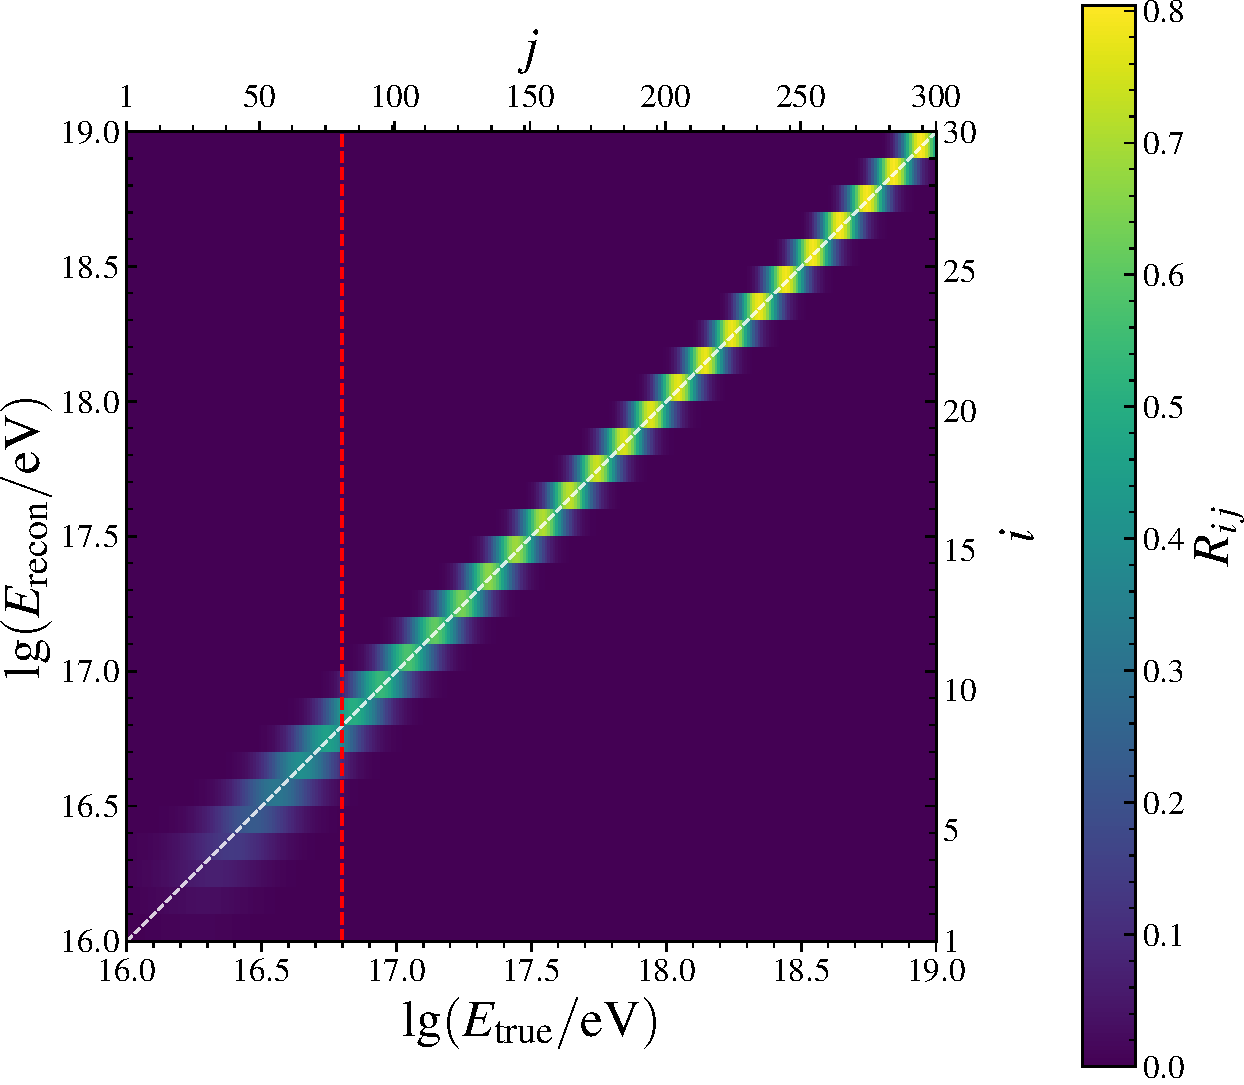
\includegraphics[width=0.75\linewidth]{figures/chapter_spectrum/sd433_migration_matrix.pdf}
    \caption{
        Approximate migration matrix for the \sd{433}.
        The horizontal axis represents true energy and the vertical axis reconstructed energy.
        The red dashed line indicates the full-efficiency threshold in true energy, and the white dashed line indicates
        $E_{\mathrm{rec}}=E_{\mathrm{true}}$.
    }
    \label{fig:migration_matrix}
\end{figure}

The efficiency suppresses the contribution from energies below the full-efficiency threshold.
Nevertheless, upward migrations allow events from up to two bins below the full-efficiency threshold to contribute significantly to the measured spectrum.
At low energies, the worsening energy resolution broadens the migration pattern, increasing the contributions from more distant true-energy bins.
At high energies, where shower-to-shower fluctuations dominate the relative energy resolution, the shape of the migration pattern becomes approximately independent of energy.

To assess the accuracy of the approximation, a power-law spectrum
\begin{align}
    J(E)=J_0E^\gamma
\end{align}
with spectral index $\gamma=-3$ is used.
The expected event numbers are calculated using both the exact matrix,
$R_{ij}^{\mathrm{exact}}$, and the approximate matrix,
$R_{ij}^{\mathrm{approx}}$.
The relative difference,
\begin{align}
    \delta\nu_i
    =
    \frac{
        \nu_i^{\mathrm{approx}}
        -
        \nu_i^{\mathrm{exact}}
    }{
        \nu_i^{\mathrm{exact}}
    },
\end{align}
is shown in \cref{fig:nu_ratio}.

\begin{figure}
    \centering
    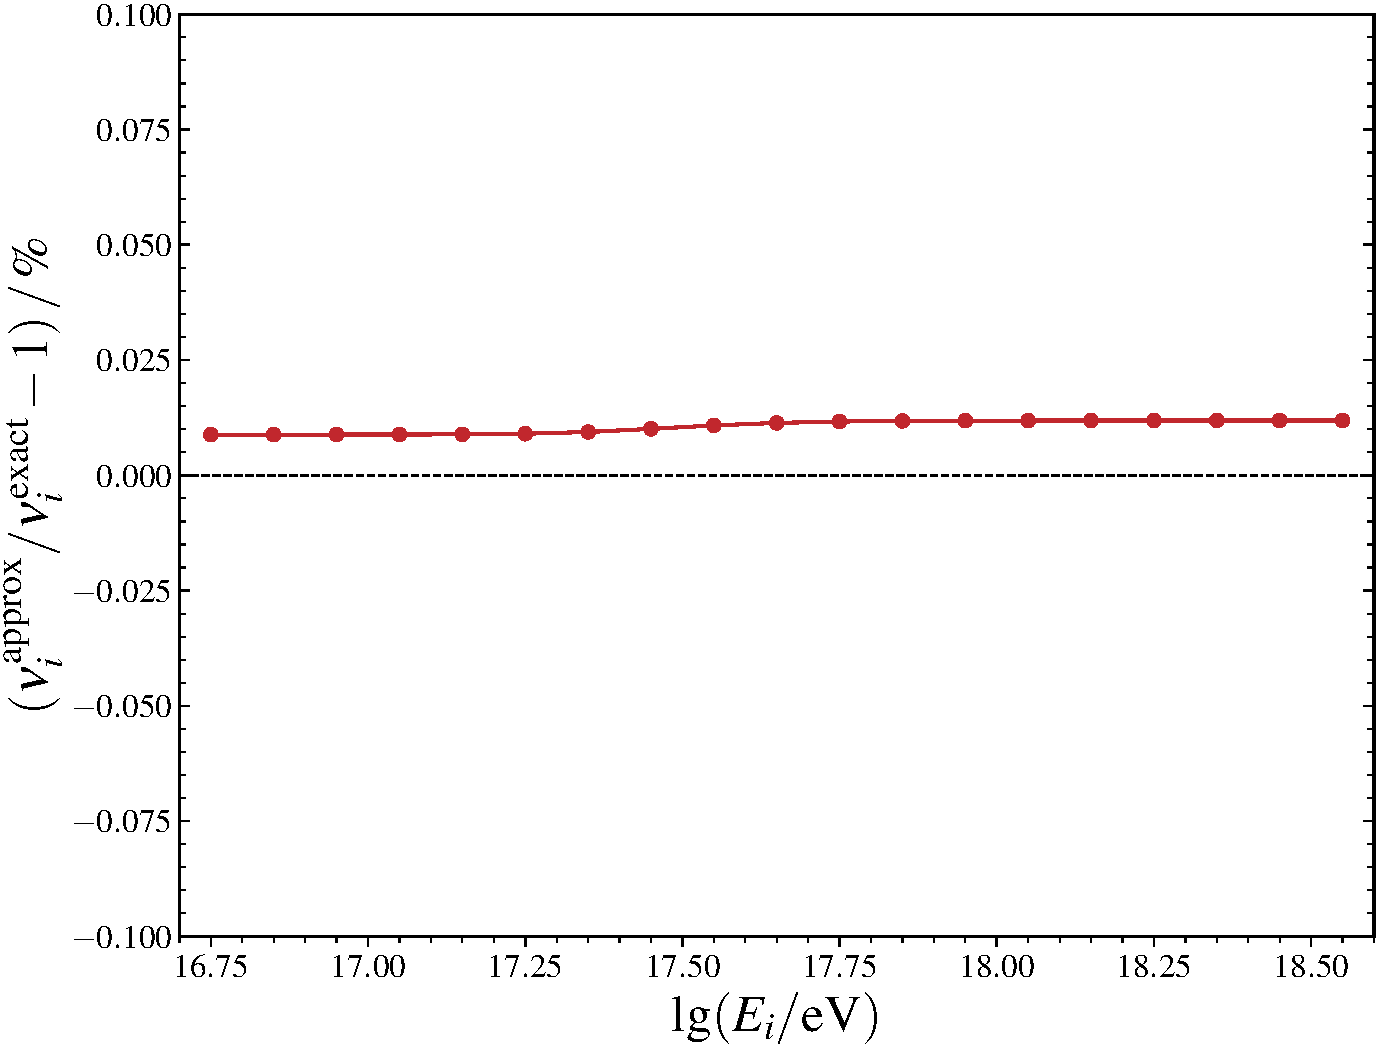
\includegraphics[width=0.75\linewidth]{figures/chapter_spectrum/nu_ratio.pdf}
    \caption{
        Relative difference between the expected event numbers obtained using the approximate and exact migration matrices for a power-law spectrum with $\gamma=-3$.
    }
    \label{fig:nu_ratio}
\end{figure}

The difference remains below $0.02\%$ over the full energy range, showing that the effect of the approximation is negligible for the chosen binning.
The approximate matrix is therefore used in the forward-folding fit, avoiding both an a priori dependence on the spectral parameters and the need to recalculate the matrix at every iteration.

Once the best-fit spectrum parameters $\hat{\mathbf{s}}$ are determined, the ratio
\begin{align}
    c_i
    =
    \frac{
        \mu_i(\hat{\mathbf{s}})
    }{
        \nu_i(\hat{\mathbf{s}})
    },
    \label{eq:correction_factor}
\end{align}
is calculated for each bin.
These correction factors are then used to estimate the true flux:
\begin{align}
    J_i
    =
    c_i J_i^{\mathrm{raw}}.
\end{align}

The resulting values for the measured \sd{433} dataset are shown in
\cref{fig:correction_factors}.
The correction factors are more relevant near the full-efficiency threshold, where the efficiency and energy resolution have the greatest impact on the measured spectrum.
At high energies, they become approximately constant because shower-to-shower fluctuations dominate the energy resolution.
\begin{figure}
    \centering
    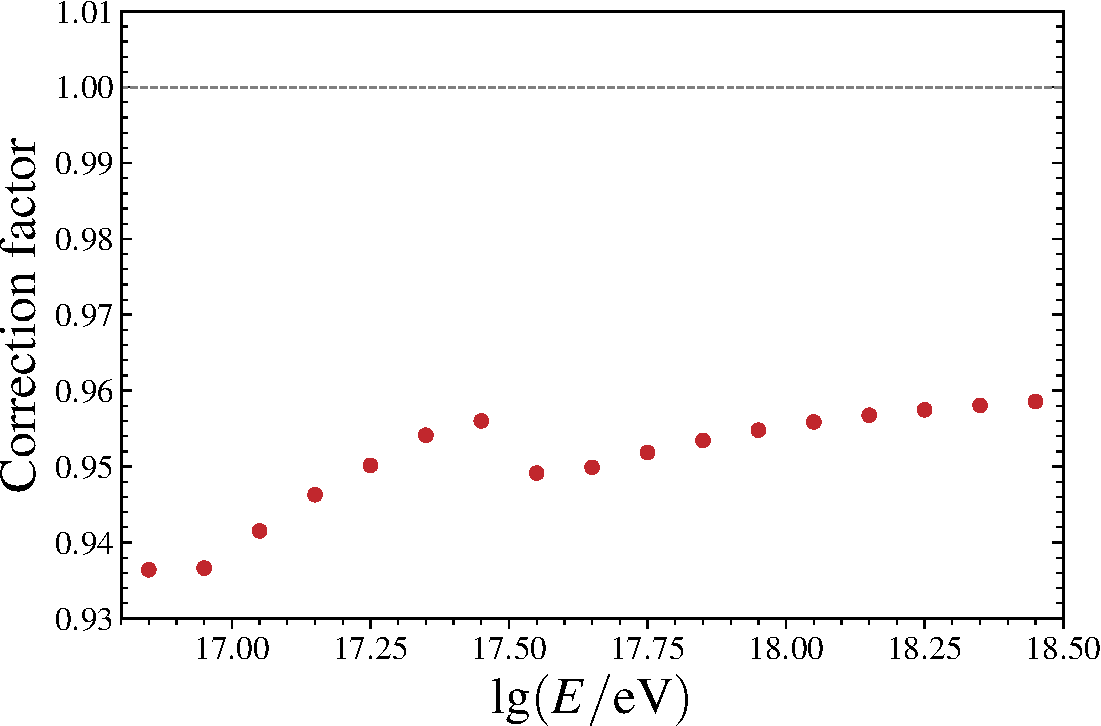
\includegraphics[width=0.75\linewidth]{figures/chapter_spectrum/sd433_nominal_correction_factors.pdf}
    \caption{
        Correction factors obtained from the forward-folding fit to the measured \sd{433} dataset.
    }
    \label{fig:correction_factors}
\end{figure}

%%%%%%%%%%%%%%%%%%%%%%%%%%%%%%%%%%%%%%%%%%%%%%%%%%%%%%%%%%%%%%%%%%%%%%%%%%%
\section{The \sd{433} Unfolded spectrum}
\label{sec:unfolded_spectrum}
%%%%%%%%%%%%%%%%%%%%%%%%%%%%%%%%%%%%%%%%%%%%%%%%%%%%%%%%%%%%%%%%%%%%%%%%%%%

Using the forward-folding procedure developed in the previous section, the \sd{433} spectrum is measured between $\lg(E/\mathrm{eV})=16.8$ and $18.5$.
The lower limit is determined by the full-efficiency threshold, and the upper limit is chosen below the ankle so that the second knee can be determined without requiring an additional spectral feature.

To test the presence of a knee-like structure in the spectrum, the data are first fitted with a simple power law,
\begin{align}
    J(E)
    =
    J_0
    \left(
        \frac{E}{10^{17}\,\mathrm{eV}}
    \right)^{-\gamma},
\end{align}
where the normalization $J_0$ and spectral index $\gamma$ are free parameters.
The resulting fit, shown in \cref{app:chap_spectrum}, yields a Poisson deviance of
$D/\mathrm{dof}=\SDFourThreeThreePowerLawDeviance/\SDFourThreeThreePowerLawDof$,
corresponding to a $p$-value of $\SDFourThreeThreePowerLawPValue$.
The simple-power-law hypothesis is therefore rejected, providing strong evidence for a change in the spectral slope within the measured energy range.
As a consequence, a broken power law with a soft transition is used to fit the spectrum,
\begin{align}
    J(E)=J_0\left(
    \frac{E}{10^{17}\,\mathrm{eV}}
    \right)^{-\gamma_0}
    \left[
    1+\left(
    \frac{E}{E_{01}}
    \right)^{\frac{1}{\omega_{01}}}
    \right]^{(\gamma_0-\gamma_1)\omega_{01}},
    \label{eq:bplwst}
\end{align}
where $J_0$ is the normalization at $10^{17}\,\mathrm{eV}$.
The second knee is characterized by its energy $E_{01}$, the spectral indices $\gamma_0$ and $\gamma_1$ before and after the feature, respectively, and $\omega_{01}$, which governs the width of the transition~\cite{PierreAuger:2021:InfillSpectrum}.

The spectrum is first fitted with all five parameters left free.
The fit converges and yields a Poisson deviance of
$D/\mathrm{dof}=12.32/12$, corresponding to a $p$-value of $0.421$.
The fitted parameters are listed in \cref{table:sd433_fits_omega}.
Although the second-knee energy and spectral indices are well constrained, the transition width is reconstructed as
$\omega_{01}=0.092\pm0.267$.
The uncertainty is considerably larger than the fitted value, and the corresponding symmetric interval includes unphysical negative values, indicating that the \sd{433} data cannot constrain the width of the transition.

\begin{table}
    \centering
    \caption{
        Spectral parameters and fit quality for the \sd{433} spectrum obtained with $\omega_{01}$ free
        and fixed to $0.05$ together with the Hess statistical uncertainties.
    }
    \label{table:sd433_fits_omega}
    \begin{tabular}{lcc}
        \hline
        Parameter
        & Free $\omega_{01}$
        & Fixed $\omega_{01}=0.05$ \\
        \hline
        $J_0/
        \left(
        10^{-13}\,
        \mathrm{km^{-2}\,yr^{-1}\,sr^{-1}\,eV^{-1}}
        \right)$
        & $0.9129\pm0.0069$
        & $0.9125\pm0.0054$ \\
        $\lg(E_{01}/\mathrm{eV})$
        & $17.438\pm0.087$
        & $17.440\pm0.083$ \\
        $\gamma_0$
        & $3.034\pm0.026$
        & $3.036\pm0.017$ \\
        $\gamma_1$
        & $3.342\pm0.078$
        & $3.342\pm0.078$ \\
        $\omega_{01}$
        & $0.092\pm0.267$
        & $0.05$ (fixed) \\
        $D/\mathrm{dof}$
        & $12.32/12$
        & $12.33/13$ \\
        $p$-value
        & $0.421$
        & $0.501$ \\
        \hline
    \end{tabular}
\end{table}

Both fits provide good descriptions of the data.
Leaving the transition width free changes the deviance by only $0.02$, despite introducing an additional fit parameter.
The reconstructed second-knee energy and spectral indices are compatible between the two fits and differ by much less than their Hesse uncertainties.
Therefore, the inability to constrain $\omega_{01}$ does not significantly affect the determination of the other spectral parameters.
Consequently, the transition width is fixed to $\omega_{01}=0.05$ for the spectrum measurement using the \sd{433} alone.
The same value was adopted by the Pierre Auger Observatory for spectral features whose transition widths could not be constrained~\cite{PierreAuger:2020:Spectrum}.
Although subdominant, the influence of $\omega_{01}$ on the measured spectrum is examined further in \cref{subsec:transition_systematic}, together with the other sources of systematic uncertainty.

With the fixed value of the transition width, the forward-folded fit was performed once more, obtaining an energy of \secondKneeEnergy, \gammaZero and \gammaOne.

The resulting unfolded spectrum and the residuals with respect to the fitted model are shown in \cref{fig:sd433_unfolded_spectrum}.
\begin{figure}
    \centering
    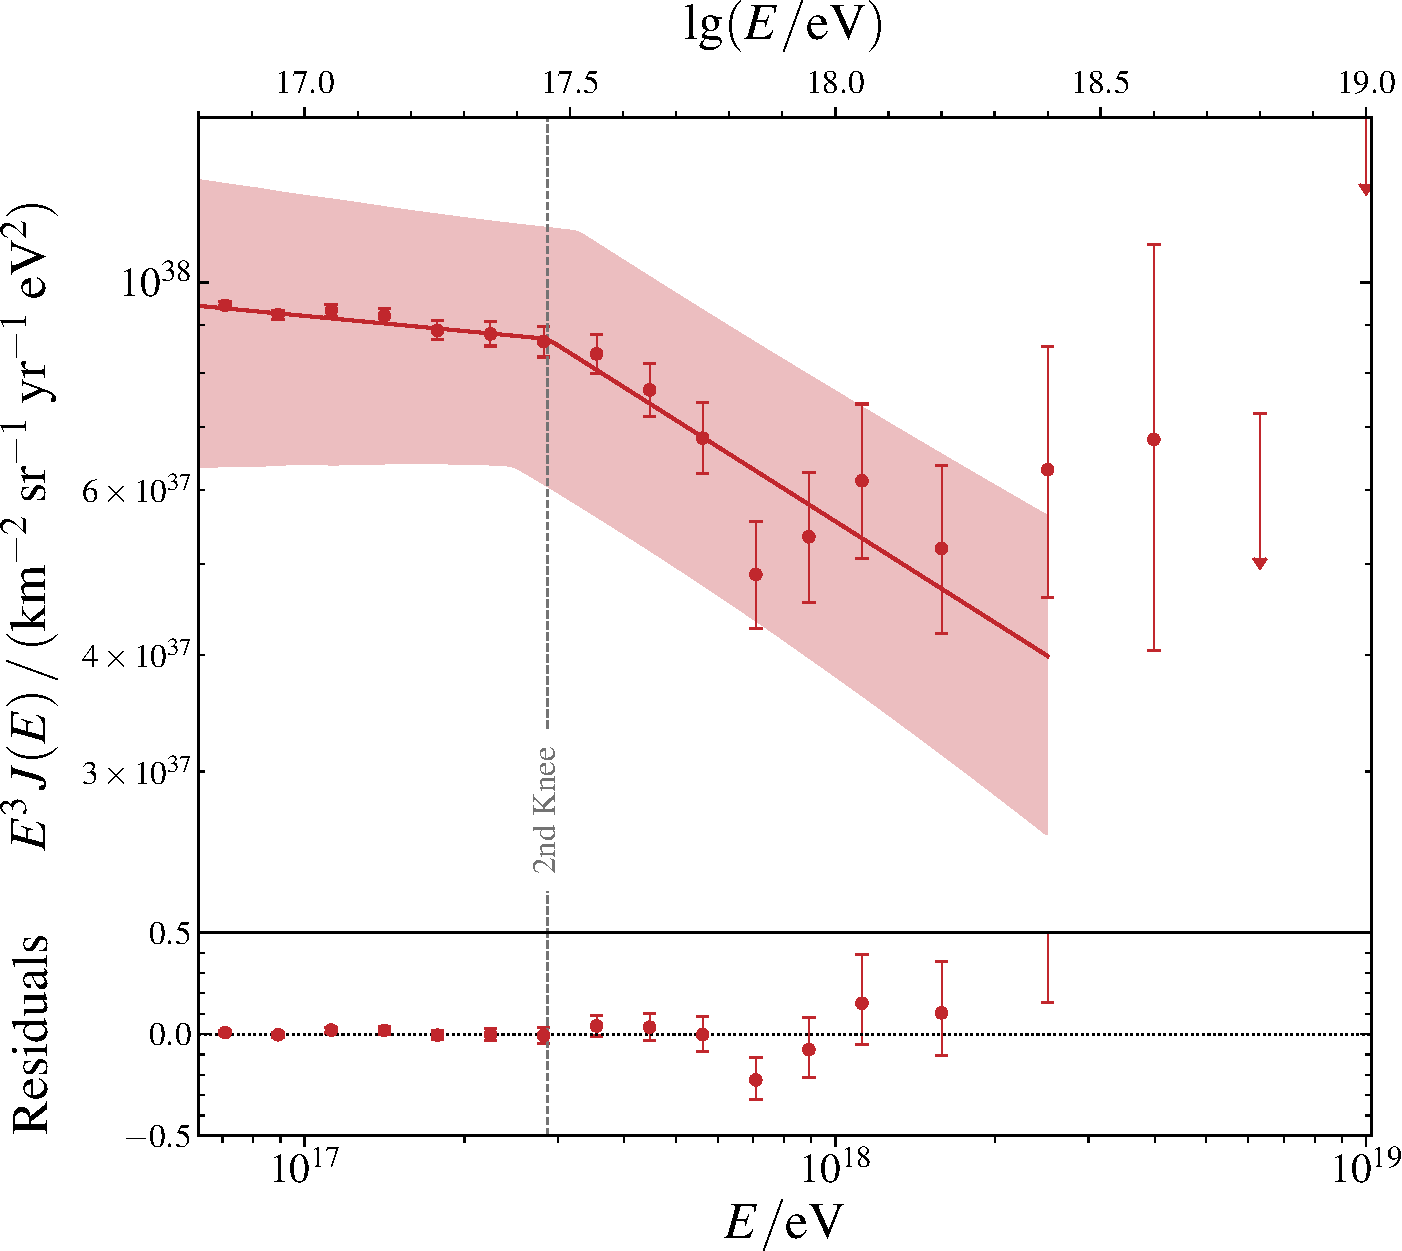
\includegraphics[width=0.8\linewidth]{figures/chapter_spectrum/sd433_unfolded_spectrum_with_residuals.pdf}
    \caption{Unfolded cosmic-ray spectrum measured with the \sd{433} and the best-fit broken power law with a smooth transition. The lower panel shows the residuals with respect to the fitted model.}
    \label{fig:sd433_unfolded_spectrum}
\end{figure}

To assess the stability of the spectral parameters, the fit was repeated by progressively increasing the minimum energy from
$\lg(E_{\min}/\mathrm{eV})=16.8$ to $17.2$.
The results are shown in \cref{fig:sd433_fit_min_stability}.
The reconstructed second-knee energy and spectral indices remain compatible within statistical uncertainties over the complete range.
As the minimum energy increases, the number of events and the lever arm below the second knee decrease.
Consequently, the uncertainty in $\gamma_0$ increases and the fit quality decreases, although the fitted value remains compatible with the nominal result.

\begin{figure}
    \centering
    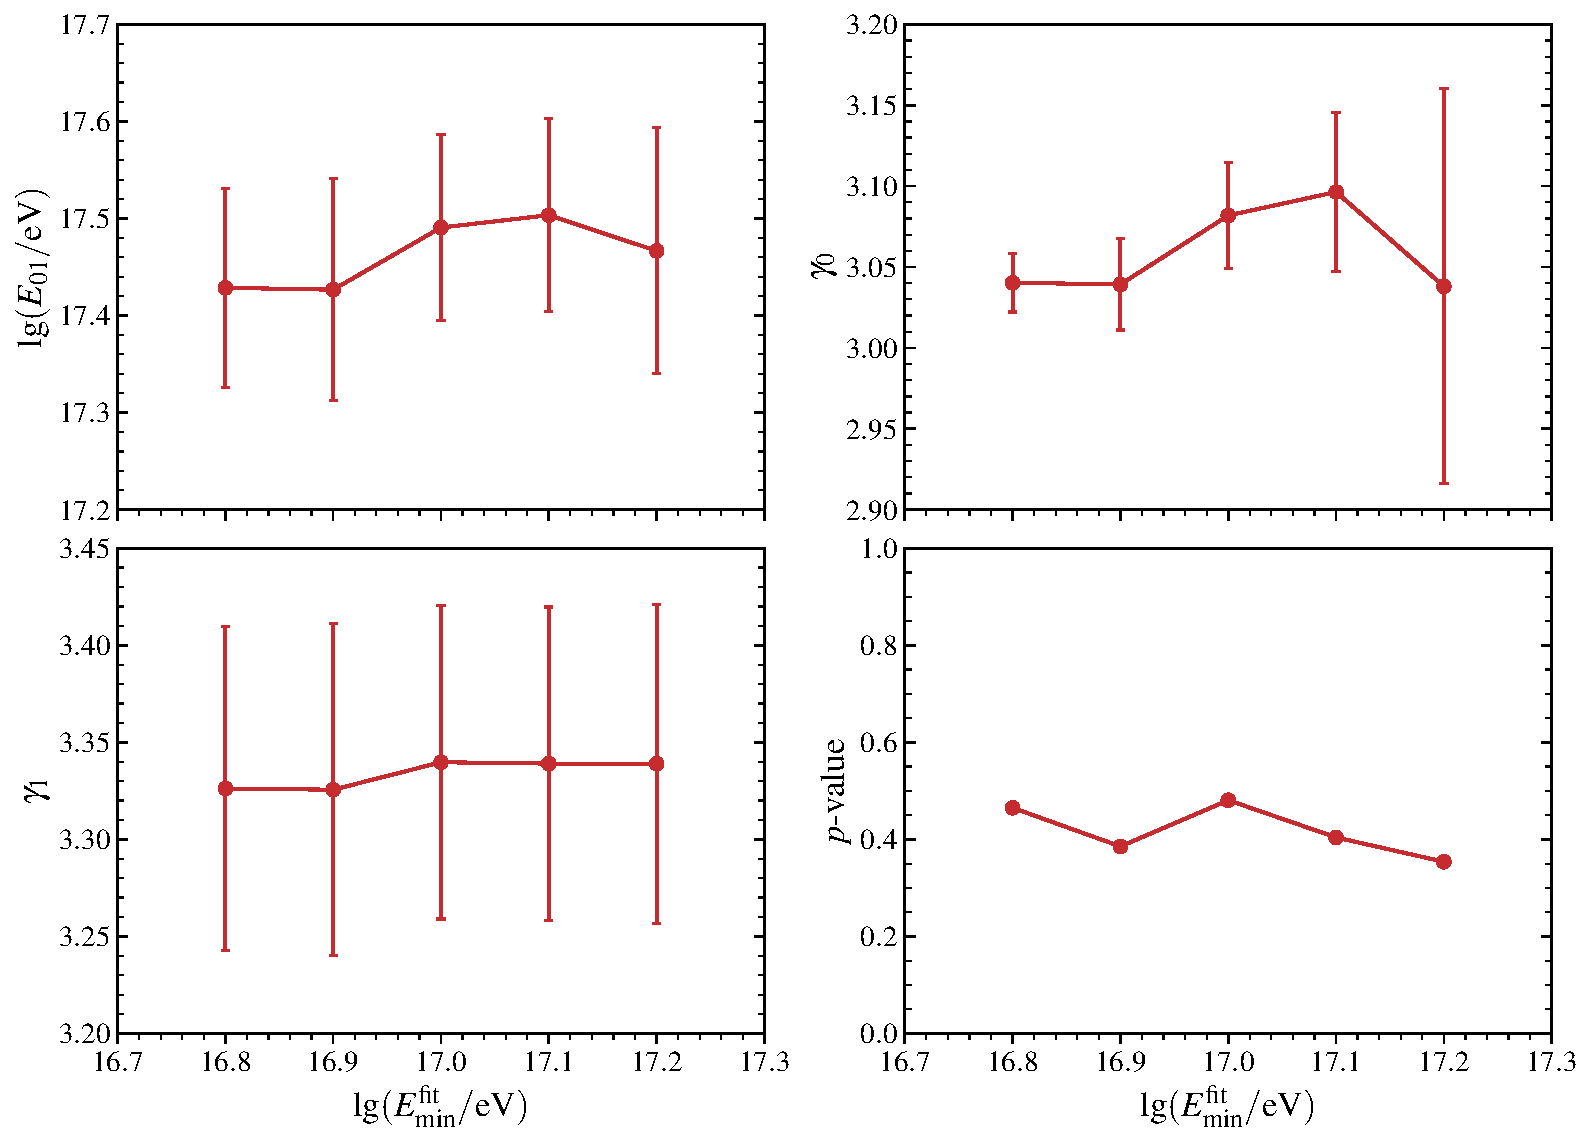
\includegraphics[width=\linewidth]
    {figures/chapter_spectrum/sd433_fit_min_stability_2x2.pdf}
    \caption{
        Dependence of the fitted second-knee parameters and Poisson deviance per degree of freedom on the minimum energy included in the fit.
        The error bars represent the statistical uncertainties of the fitted parameters.
    }
    \label{fig:sd433_fit_min_stability}
\end{figure}

%%%%%%%%%%%%%%%%%%%%%%%%%%%%%%%%%%%%%%%%%%%%%%%%%%%%%%%%%%%%%%%%%%%%%%%%%%%
\section{Spectrum systematics}
\label{sec:systematics}
%%%%%%%%%%%%%%%%%%%%%%%%%%%%%%%%%%%%%%%%%%%%%%%%%%%%%%%%%%%%%%%%%%%%%%%%%%%

The systematic uncertainties affecting the \sd{433} spectrum arise from the exposure, the energy scale, the detector response, and the assumed transition width.
The dominant contribution is the approximately $14\%$ energy-scale uncertainty inherited from the calibration of the \sd{750} with the FD.

The exposure uncertainty is approximately $3\%$ and is energy independent, since the exposure is calculated geometrically from the number of active hexagons~\cite{PierreAuger:2010:TriggerAperture}.
The uncertainties associated with the detector response include the energy resolution and the composition dependence of the bias and efficiency.
The uncertainties in the calibration parameters determined in \cref{chapter:reconstruction} are also included.

These sources are treated as uncorrelated, and their effects on both the flux and the fitted spectral parameters are evaluated using the forward-folding procedure developed in the previous section.
Their contributions are combined in quadrature to determine the total systematic uncertainty of the measurement.
The influence of the assumed value of $\omega_{01}$ on the determination of the second knee is assessed separately using the measured data and toy Monte-Carlo simulations.

\subsection{FD energy systematic}

The calibration of the \gls{sd} with the \gls{fd} transfers the systematic uncertainty of the FD energy scale to the \sd{433} spectrum.
The individual contributions to this uncertainty are described in detail in \cite{PierreAuger:2015:Observatory} and summarized in \cref{table:energy_scale_systematics}.
The dominant contributions arise from the absolute calibration of the \gls{fd} and the reconstruction of the longitudinal shower profile.

\begin{table}
    \centering
    \caption{Contributions to the systematic uncertainty in the \gls{fd} energy scale.
    The ranges indicate the energy dependence of the corresponding contributions.
    The total uncertainty amounts to 14\,\%.}
    \label{table:energy_scale_systematics}
    \begin{tabular}{lr}
        \hline
        Fluorescence yield
            & 3.6\,\% \\
        Atmosphere
            & 3.4--6.2\,\% \\
        FD calibration
            & 9.9\,\% \\
        FD profile reconstruction
            & 5.6--6.5\,\% \\
        Invisible energy
            & 3--1.5\,\% \\
        Statistical error of SD calibration fit
            & 0.7--1.8\,\% \\
        Stability of the energy scale
            & 5\,\% \\
        \hline
        \textbf{Total}
            & \textbf{14\,\%} \\
        \hline
    \end{tabular}
\end{table}

Some contributions exhibit a mild energy dependence, while the total uncertainty is approximately energy independent and amounts to $14\%$.

The effect of the energy-scale uncertainty on the spectrum can be derived analytically.
However, the forward-folding procedure developed in the previous section is used as a cross-check.
For a relative shift $\delta$ in the energy scale, the shifted energy is $E'=(1+\delta)E$, with $\delta=\pm0.14$.
The corresponding change in the flux follows from the transformation of a probability density,
\begin{align}
    J'(E')=J(E)\left|\frac{dE}{dE'}\right|
    \label{eq:change_of_variables}
\end{align}
where $J(E)$ and $J'(E')$ are the differential fluxes on the original and shifted energy scales, respectively.
For a power-law spectrum, $J(E)=J_0E^{-\gamma}$, the relative change in the flux is
\begin{align}
\frac{\Delta J}{J}=(1+\delta)^{\gamma-1}-1,
\label{eq:energy_systematic_pl}
\end{align}
For $\gamma=3.35$, \cref{eq:energy_systematic_pl} gives flux shifts of approximately
$\SI{+36}{\percent}$ and $\SI{-30}{\percent}$ for $\delta=+0.14$ and $-0.14$, respectively.
Applying the same transformation to the smoothly broken power law in \cref{eq:bplwst} gives
\begin{align}
\frac{\Delta J(E)}{J(E)}
=
\frac{1}{1+\delta}
\frac{
J\left(\frac{E}{1+\delta}\right)
}{
J(E)
}
-1
\label{eq:energy_systematic_bplwst}
\end{align}
The analytical estimate obtained from the fitted \sd{433} spectrum is shown in
\cref{fig:energy_systematic}, together with the asymptotic limits from
\cref{eq:energy_systematic_pl}.

As a cross-check, the reconstructed energy of every event is shifted coherently by
$\delta=\pm0.14$, and the complete forward-folding and unfolding procedures are repeated.
The migration matrix is kept unchanged because the energy-scale shift does not modify the assumed detector resolution, bias, or efficiency.
The corresponding unfolded spectra are shown in
\cref{appendix_chapter_spectrum}.

The flux variations obtained with this procedure are also shown in
\cref{fig:energy_systematic}.
The forward-folding and analytical results agree over most of the energy range.
The differences around the second knee arise from the limited statistics above the feature and the resulting uncertainty in $\gamma_1$.

\begin{figure}
    \centering
    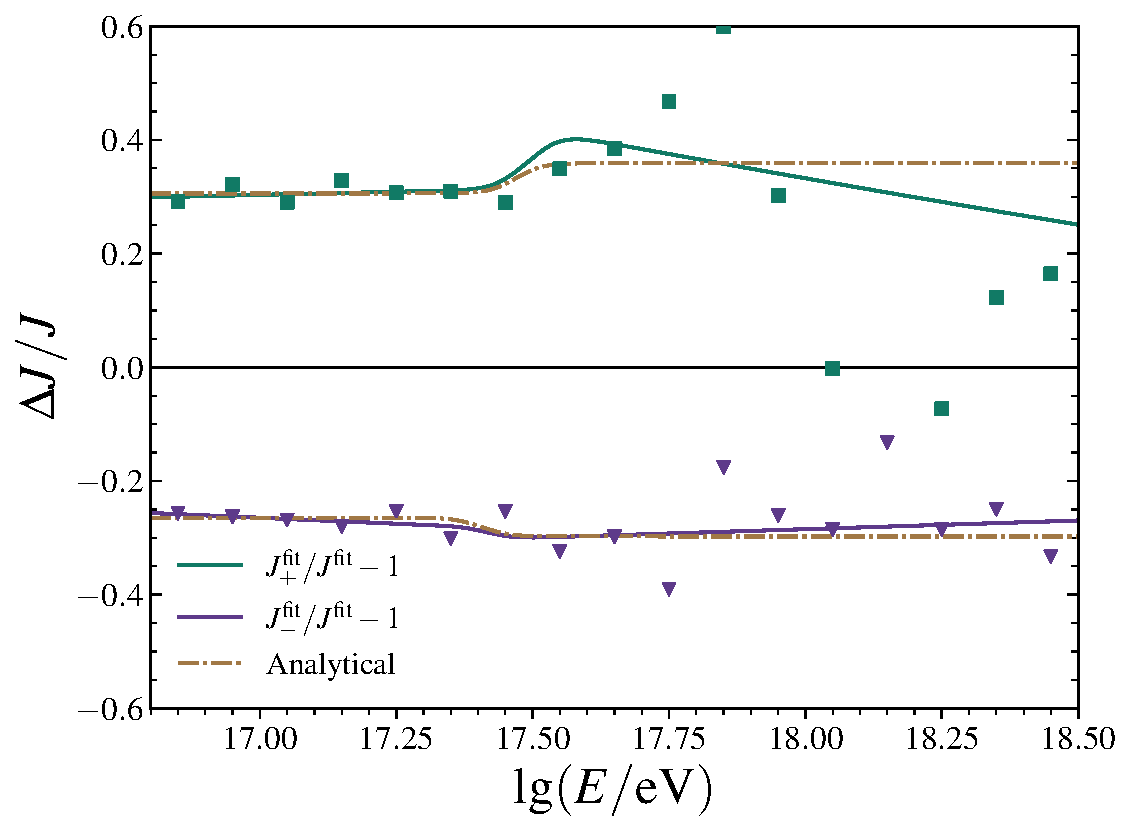
\includegraphics[width=0.8\linewidth]{figures/chapter_spectrum/delta_j_over_j.pdf}
    \caption{Relative change in the fitted flux after coherently shifting the reconstructed energies by $+14\%$ and $-14\%$. The solid curves show the result of repeating the forward-folding fit, while the dash-dotted curves show the analytical expectation from \cref{eq:energy_systematic_bplwst}. The horizontal dashed lines indicate the corresponding asymptotic simple-power-law expectations.}
    \label{fig:energy_systematic}
\end{figure}

The effect of the energy-scale shifts on the fitted spectral parameters is shown in \cref{fig:energy_systematic_fit_parameters}.
\begin{figure}
    \centering
    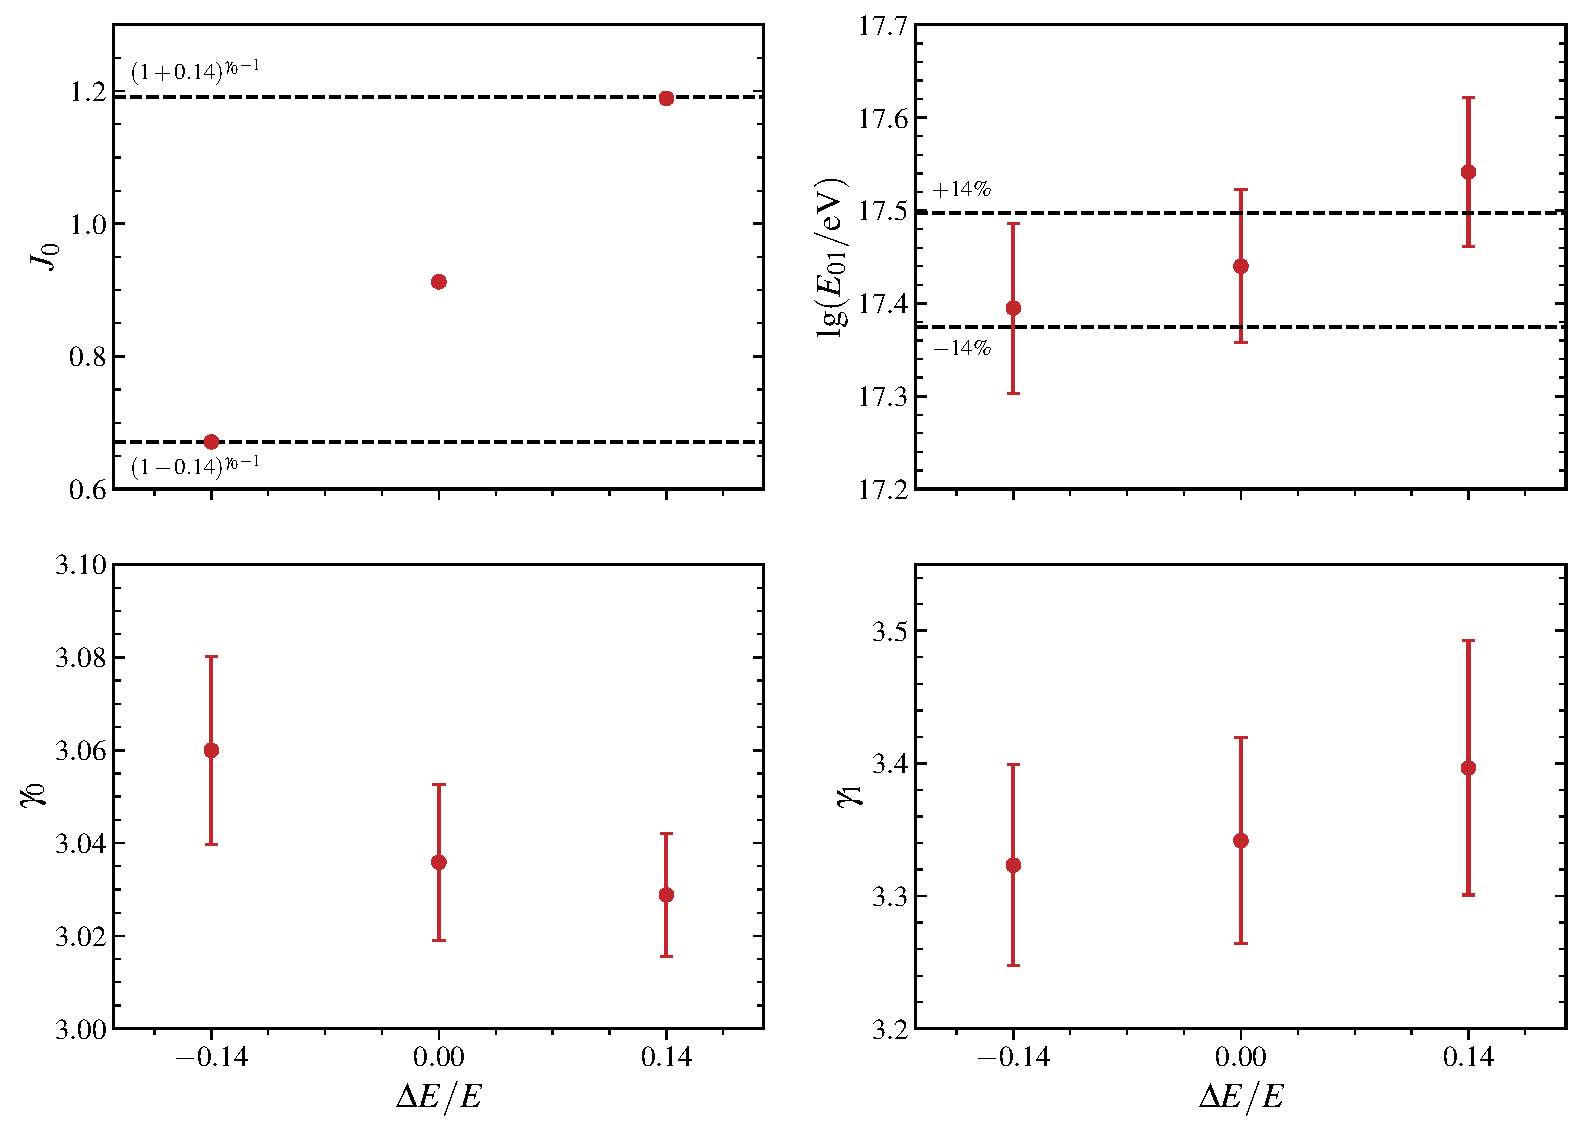
\includegraphics[width=\linewidth]{figures/chapter_spectrum/energy_systematic_fit_parameters.pdf}
    \caption{Fitted normalization $J_0$, second-knee energy $E_{01}$, and spectral indices $\gamma_0$ and $\gamma_1$ for the nominal energy scale and for coherent shifts of $+14\%$ and $-14\%$. The error bars show the statistical uncertainties of the fits. The dashed lines in the upper panels indicate the expectations obtained by directly propagating the energy-scale shift.}
    \label{fig:energy_systematic_fit_parameters}
\end{figure}

The changes in $\gamma_0$ and $\gamma_1$ are consistent with statistical uncertainties, in accordance with what is expected, given that a uniform change in energy does not impact the slope of the spectrum.
The shifts obtained from the forward-folding procedure are larger than these expectations.
Therefore, a conservative systematic uncertainty of
$\Delta\lg(E_{01}/\mathrm{eV})=0.10$ is assigned, corresponding to the largest variation obtained from the fit.


\subsection{Response function systematics}
\label{subsec:response_systematics}

The systematic uncertainties associated with the detector response are evaluated by varying the energy resolution, bias, and efficiency independently.
The contribution from the energy resolution is determined by varying the parameters of the resolution model defined in \cref{eq:resolution_sigma}, following the procedure in \cite{PierreAuger:2021:InfillSpectrum}.
The parameters $R_{\mathrm{sh}}$ and $R_0$ are shifted by their respective $1\sigma$ uncertainties, corresponding to variations of $\pm0.01$ for each parameter.
For each variation, the migration matrix is recalculated while keeping the other components of the detector response unchanged, and the spectrum is fitted again.
The spectral-shape parameters remain well within their nominal statistical uncertainties. 
For each source of systematic uncertainty, the contribution to $\Delta J/J$ was calculated as the root mean square of the relative flux variations.
The resulting contribution from the energy resolution is shown in the left panel of \cref{fig:sd433_systematic_budget}.
Its magnitude is largest near the full-efficiency threshold, where it reaches approximately $1.1\%$, and decreases with energy.
Increasing the resolution parameters lowers the reconstructed flux, whereas decreasing them raises it.  
The resulting spectra and fitted parameters are reported in \cref{appendix_chapter_spectrum}.

The dependence of the detector response on the assumed mass composition is estimated using the bias and efficiency parametrizations obtained in \cref{sec:res_and_bias} for pure proton and pure iron primaries.
The bias and efficiency contributions are evaluated separately, following the same procedure used for the resolution uncertainty.

The bias variations leave the position of the second knee and the spectral indices essentially unchanged.
However, their contribution to $\Delta J/J$ reaches approximately $4.3\%$ near the full-efficiency threshold.

The composition dependence of the efficiency produces a smaller contribution to the flux uncertainty, with a maximum of approximately $1.5\%$.
Nevertheless, it shifts the position of the second knee downward by
$\Delta\lg(E_{01}/\mathrm{eV})=-0.03$.

The contributions from the composition dependence of the bias and efficiency are shown in the left panel of \cref{fig:sd433_systematic_budget}.

\subsection{Calibration systematic}
\label{subsec:calibration_systematic}

The energy assigned to each \sd{433} event is obtained from its calibration with the \sd{750} energy estimator, described in \cref{sec:calibration}.
In addition to the uncertainty inherited from the FD energy scale, the finite precision of this calibration introduces an independent contribution to the spectrum uncertainty.
This contribution arises from the uncertainties in the normalization $A$ and slope $B$ of the calibration relation.
A variation of $A$ produces a uniform shift in energy, whereas a variation of $B$ produces an energy-dependent shift and can therefore modify the spectral indices.

The effect of the calibration slope can be understood analytically.
For the calibration relation
\begin{align}
    E=A\left(\frac{S_{30}}{S_0}\right)^B,
\end{align}
a normalization $A=\SDFourThreeThreeCalA$, a slope $B=\SDFourThreeThreeCalB$, and a reference signal $S_0=\SDFourThreeThreeCalSZero$ are used in the frozen reconstruction.
A change from $B$ to $B'$, while keeping $A$ fixed, transforms the reconstructed energy according to
\begin{align}
    E'
    =
    A
    \left(\frac{E}{A}\right)^{\frac{B'}{B}}.
    \label{eq:calibration_energy_transformation}
\end{align}
The corresponding transformation of the flux follows from the change of variables in \cref{eq:change_of_variables},
\begin{align}
    J'(E')
    =
    \frac{B}{B'}
    \frac{E}{E'}
    J(E).
    \label{eq:calibration_flux_transformation}
\end{align}
For a power law spectrum, $J(E)\propto E^{-\gamma}$, the transformed spectrum is also a power law with spectral index
\begin{align}
    \gamma'
    =
    1+(\gamma-1)\frac{B}{B'}.
    \label{eq:calibration_spectral_index}
\end{align}
This yields a change in the spectral index
\begin{align}
    \Delta\gamma
    =
    (\gamma-1)
    \left(\frac{B}{B'}-1\right).
    \label{eq:calibration_spectral_index_change}
\end{align}
Consequently, the uncertainty in $A$ produces a uniform shift in the energy scale, affecting the flux normalization and the position of spectral features, whereas the uncertainty in $B$ modifies the shape of the reconstructed spectrum.

In the systematic evaluation, the calibration parameters are varied according to the systematic uncertainties determined in \cref{sec:calibration}.
The correlated variations used to define the systematic envelope are
$(A^+,B^-)=(125.7~\mathrm{PeV},0.909)$ and
$(A^-,B^+)=(113.3~\mathrm{PeV},0.983)$.
The nominal and varied calibration relations are shown in the left panel of
\cref{fig:calibration_systematic}.
For each variation, the energy of every event is recalculated and the spectrum is fitted again.
The resulting unfolded spectra are shown in the right panel.
\begin{figure}
    \centering
    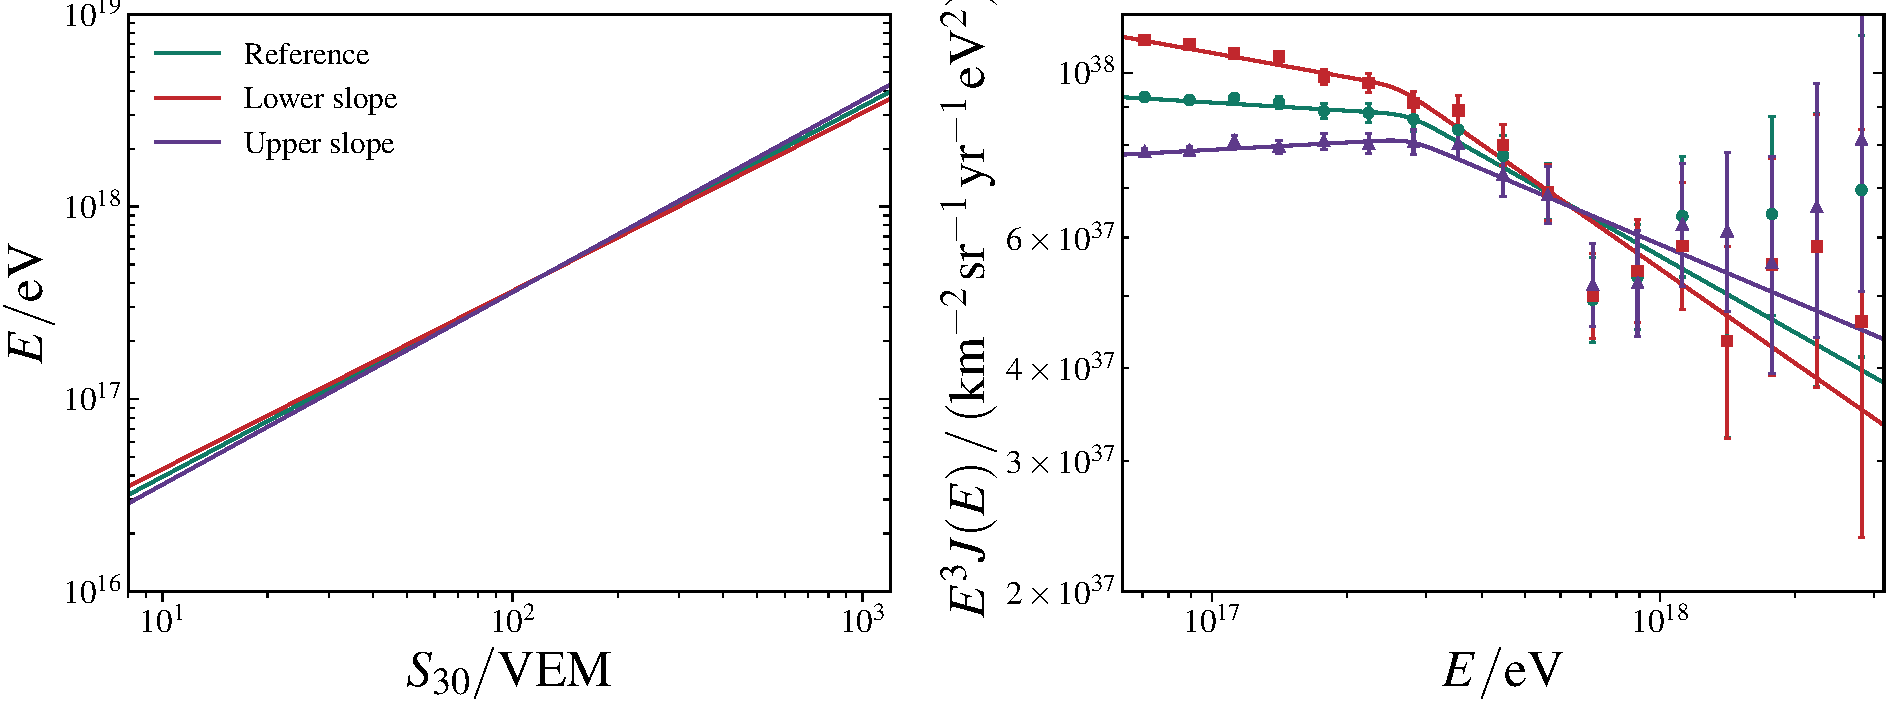
\includegraphics[width=\textwidth]{figures/chapter_spectrum/calibration_systematic.pdf}
    \caption{
        Effect of the calibration systematic on the reconstructed spectrum.
        The left panel shows the reference calibration relation together with the lower- and upper-slope variations.
        The right panel shows the corresponding unfolded spectra scaled by $E^3$ together with their respective fitted spectral functions.
    }
    \label{fig:calibration_systematic}
\end{figure}
Using the nominal fit values, $\gamma_0=3.036$ and $\gamma_1=3.342$,
\cref{eq:calibration_spectral_index_change} predicts
$\Delta\gamma_0^{\mathrm{analytical}}=0.083$ and
$\Delta\gamma_1^{\mathrm{analytical}}=0.095$.
The corresponding changes obtained from the spectrum fit are
$\Delta\gamma_0^{\mathrm{fit}}=0.073$ and
$\Delta\gamma_1^{\mathrm{fit}}=0.081$.
The fitted changes therefore agree closely with the analytical expectations.
Since the analytical estimates are slightly larger, they are adopted as conservative systematic uncertainties.
The position of the second knee changes by at most
$\Delta\lg(E_{01}/\mathrm{eV})=0.024$, well within its statistical uncertainty.

The flux uncertainty produced by the calibration variations is shown in the right panel of \cref{fig:systematic_budget}.
It is the second-largest contribution after the energy-scale uncertainty and is also asymmetric because of the shape of the spectrum.
Its magnitude is largest at the boundaries of the energy range, reaching
$18.6\%$ at $\lg(E/\mathrm{eV})=16.8$ and
$13.4\%$ at $\lg(E/\mathrm{eV})=18.5$.
The right panel also shows the contributions from the exposure and unfolding assumptions, together with the total uncertainty obtained by combining the independent contributions in quadrature.
\begin{figure}
    \centering
    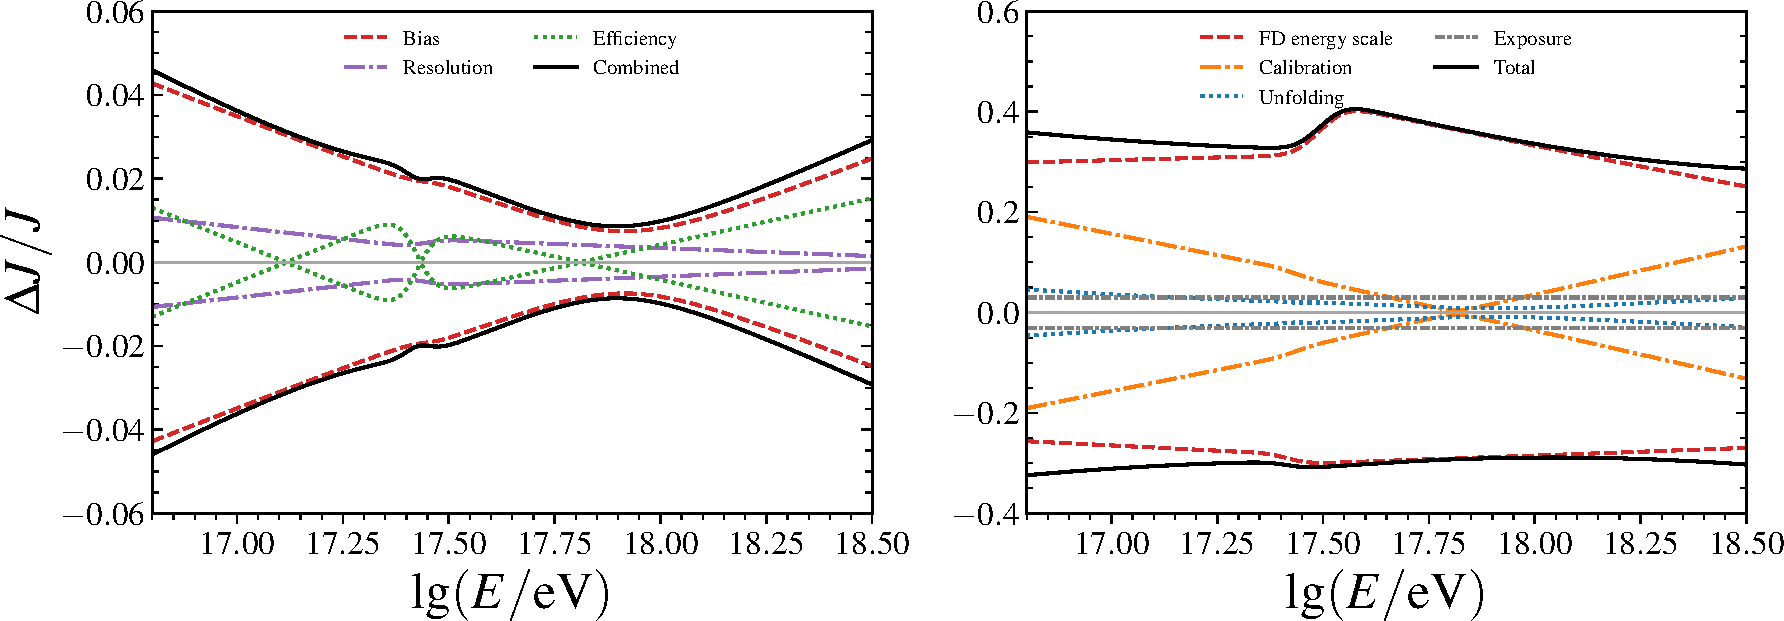
\includegraphics[width=\linewidth]{figures/chapter_spectrum/sd433_systematic_budget.pdf}
    \caption{Relative systematic uncertainty in the \sd{433} cosmic-ray flux. Left: contributions associated with the assumptions used to calculate the migration matrix, obtained by varying the energy bias, efficiency, and resolution. The black curves show their quadratic sum. Right: systematic uncertainty, including the \gls{fd} energy scale, calibration parameters, combined unfolding contribution, and exposure. The black curves show the upper and lower limits by adding the independent contributions in quadrature. }
    \label{fig:systematic_budget}
\end{figure}

\subsection{Transition systematic}
\label{subsec:transition_systematic}

As discussed in \cref{sec:unfolded_spectrum}, leaving the transition width free yields
$\omega_{01}^{\mathrm{free}}=0.092\pm0.267$.
The large uncertainty, which extends into the unphysical region of negative values, shows that the \sd{433} data cannot constrain this parameter.
Its impact on the spectrum measurement is therefore studied using toy Monte-Carlo simulations and a profile-likelihood scan of the measured data.

A total of 300 toy spectra are generated from \cref{eq:bplwst}, each containing 40,000 events to approximate the size of the measured dataset.
The detection efficiency is applied during the generation, and the energy of each event is smeared according to the response function in \cref{eq:resolution_function}.
Each toy spectrum is then fitted using the approximate migration matrix from \cref{eq:matrix_approx}.

Of the 300 toy spectra, 296 are fitted successfully.
However, 125 of these fits yield values of $\omega_{01}$ at the allowed boundaries.
The distributions of the reconstructed spectral parameters are shown in
\cref{fig:omega_monte_carlo}.
The accumulation of fitted values at the boundaries confirms that the transition width cannot be constrained with the statistics of the current \sd{433} dataset.

\begin{figure}
    \centering
    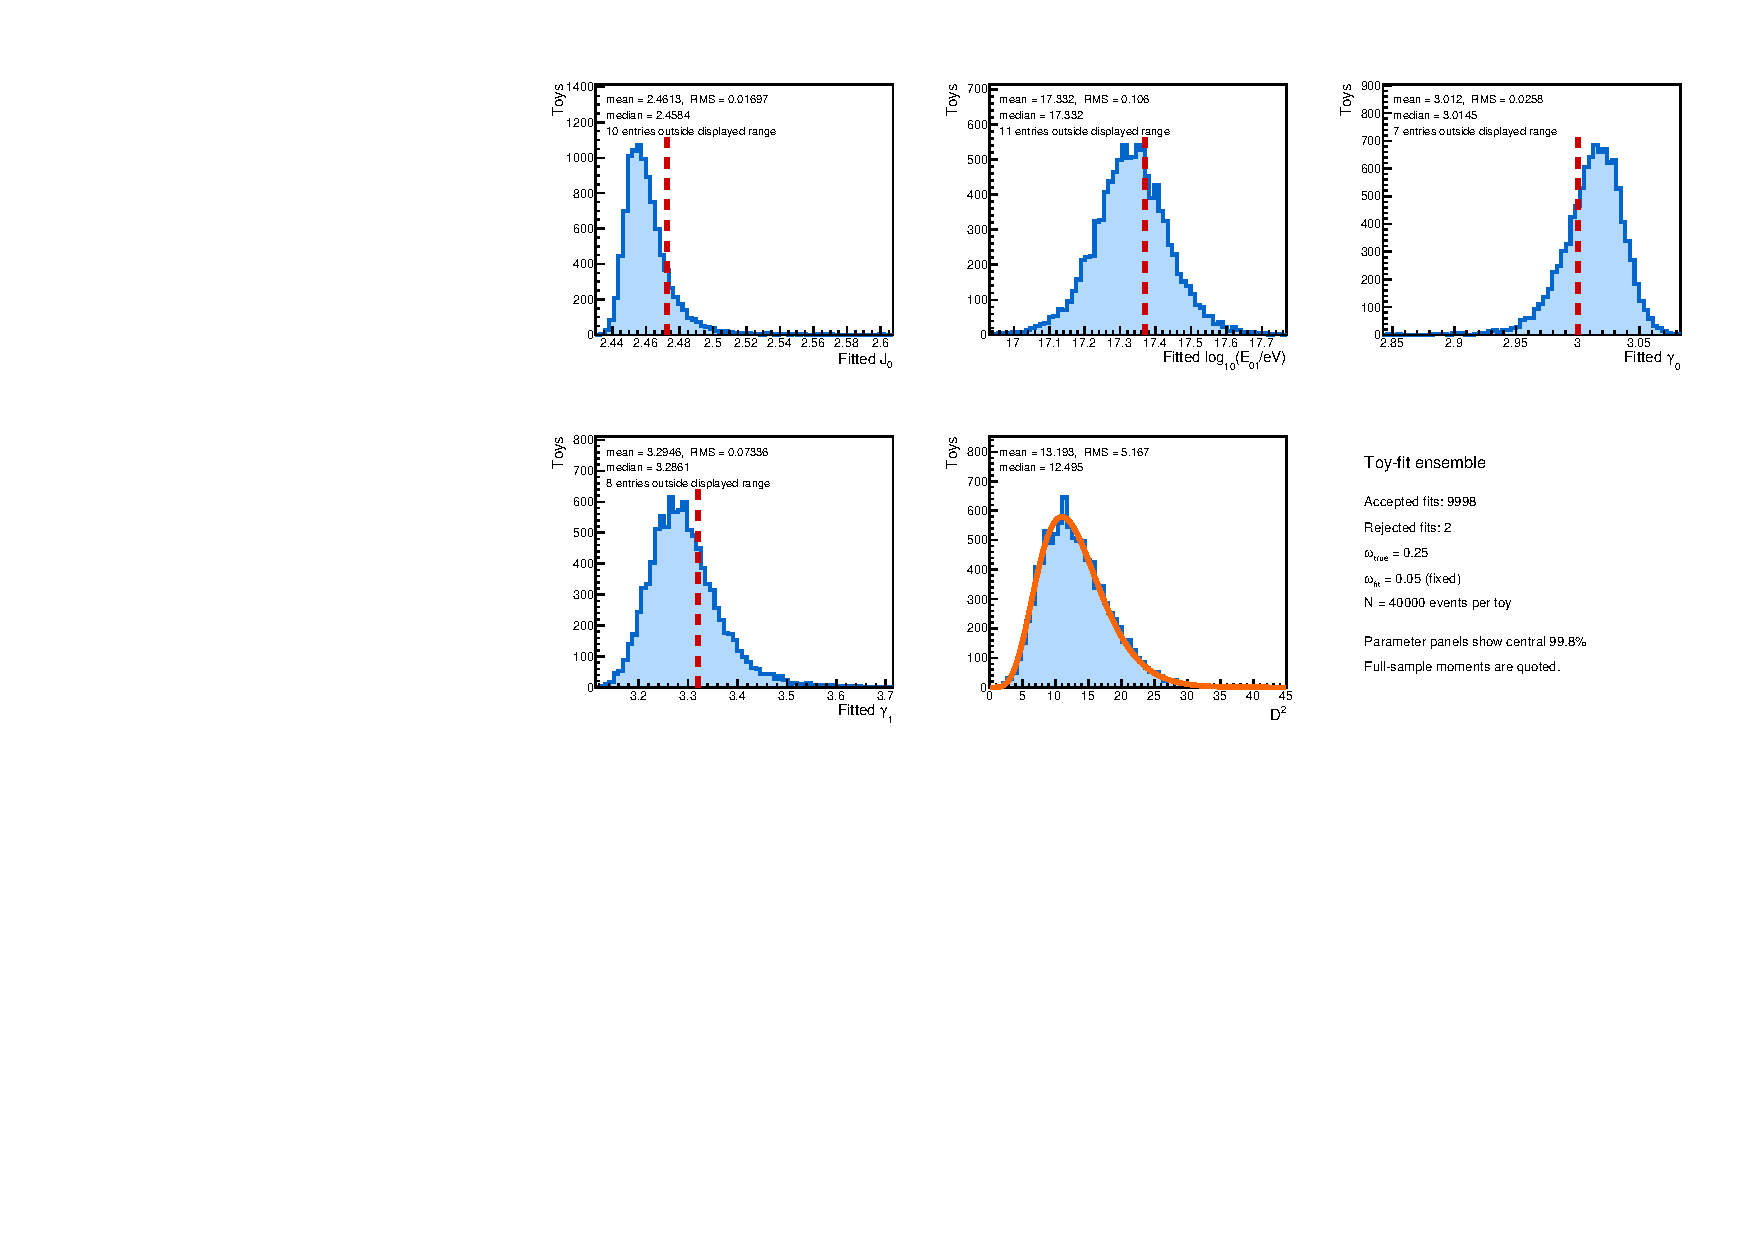
\includegraphics[width=\linewidth]{figures/chapter_spectrum/omega_free_toy_histograms.pdf}
    \caption{Distributions of the spectral parameters reconstructed from toy Monte-Carlo spectra when the transition width $\omega_{01}$ is left free. The dashed vertical lines indicate the injected values, while the solid vertical lines show the mean fitted values and the shaded regions represent the corresponding $1\sigma$ intervals.}
    \label{fig:omega_monte_carlo}
\end{figure}

To test whether fixing the transition width biases the reconstructed spectral parameters, 300 toy spectra of 40,000 events are generated with $\omega_{01}=0.25$ and fitted with $\omega_{01}=0.05$.
This deliberately compares a broad injected transition with the substantially sharper transition fixed in the fit to the measured data.
The distributions of the reconstructed second-knee energy and spectral indices are shown in \cref{fig:omega_wrong}, together with their median and injected values.
The reconstructed parameters remain compatible with the injected values within their statistical uncertainties, showing that fixing an incorrect transition width does not introduce a significant bias at the current level of statistics.

\begin{figure}
    \centering
    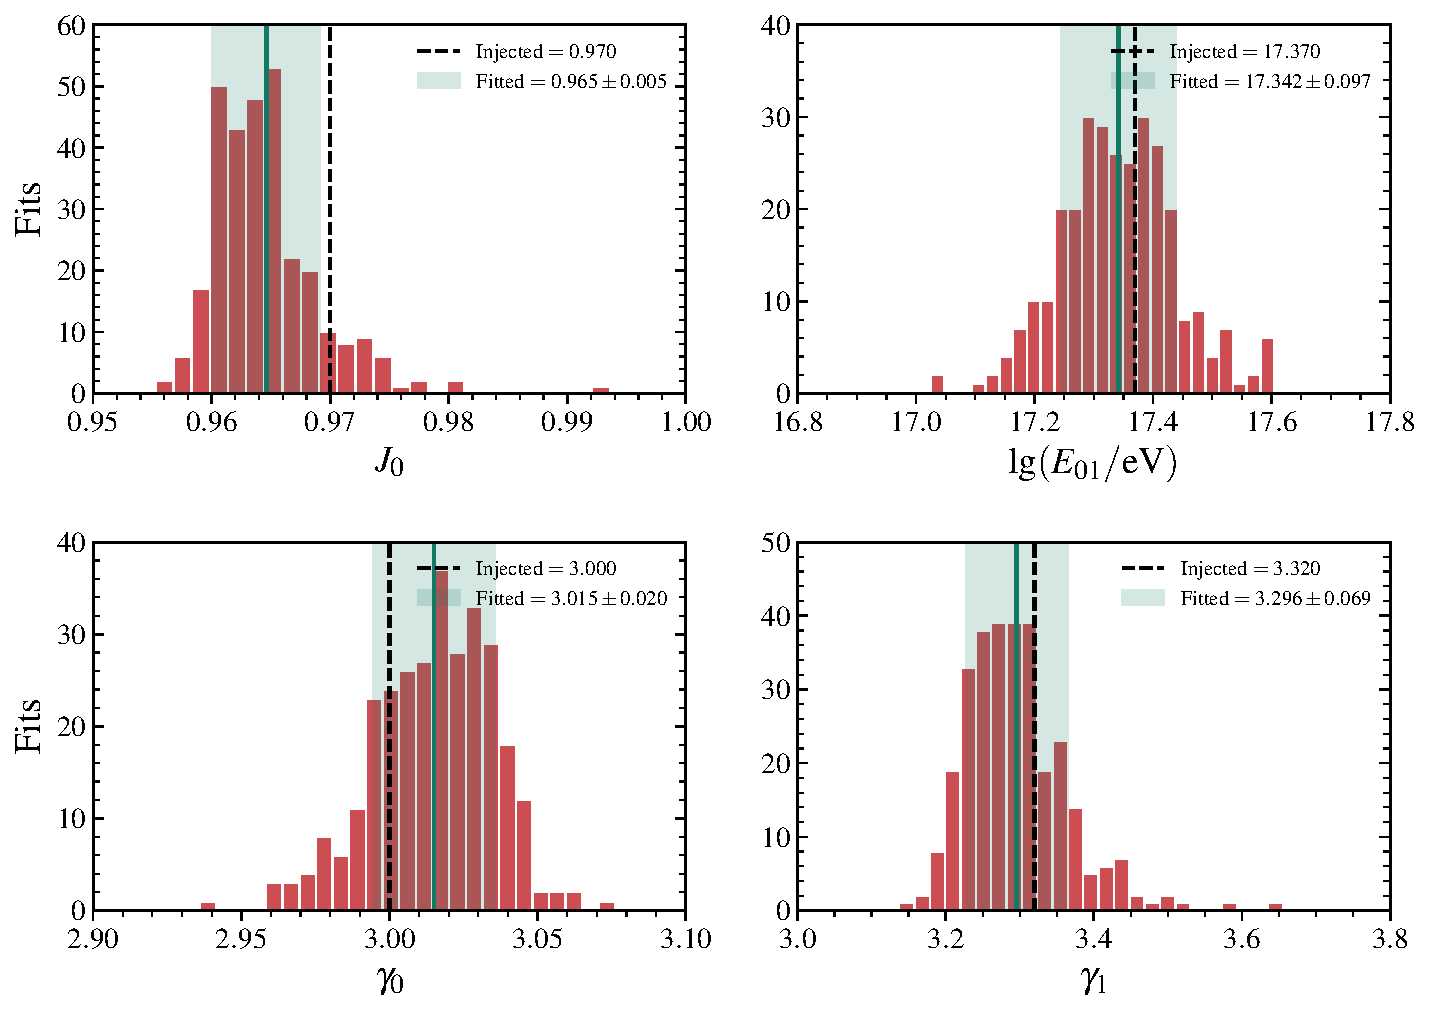
\includegraphics[width=\linewidth]{figures/chapter_spectrum/omega_wrong_closure_python.pdf}
    \caption{Distributions of the spectral parameters reconstructed from toy spectra generated with $\omega_{01}=0.25$ and fitted with a sharp transition fixed to $\omega_{01}=0.05$, as used for the measured data. The dashed vertical lines indicate the injected values, while the solid vertical lines show the mean fitted values and the shaded regions represent the corresponding $1\sigma$ intervals.}
    \label{fig:omega_wrong}
\end{figure}

To assess the effect of the assumed transition width on the other spectral parameters, the fit is repeated with $\omega_{01}$ fixed between $0$ and $0.5$ in steps of $0.05$.
The fit converges over the complete range.
The resulting Poisson deviance, second-knee energy, and spectral indices are shown in \cref{fig:omega_study}.
The circles represent the fits with fixed $\omega_{01}$, with $\omega_{01}=0$ corresponding to the sharp broken-power-law limit.
The star indicates the result obtained when $\omega_{01}$ is left free.

The deviance varies by only approximately $1.6$ over the complete scan, indicating that the \sd{433} data have little sensitivity to the transition width.
The reconstructed second-knee energy remains compatible within statistical uncertainties with the nominal result obtained for $\omega_{01}=0.05$.

A mild correlation is observed between the transition width and the spectral indices.
As $\omega_{01}$ increases, the fitted value of $\gamma_0$ decreases from approximately $3.04$ to $2.97$, while $\gamma_1$ increases from approximately $3.34$ to $3.38$.
This behaviour reflects a compensation between the transition width and the asymptotic slopes: a broader transition is accommodated by a flatter spectrum below the second knee and a steeper spectrum above it.
Nevertheless, these variations remain compatible with the statistical uncertainties of the corresponding fits.

\begin{figure}
    \centering
    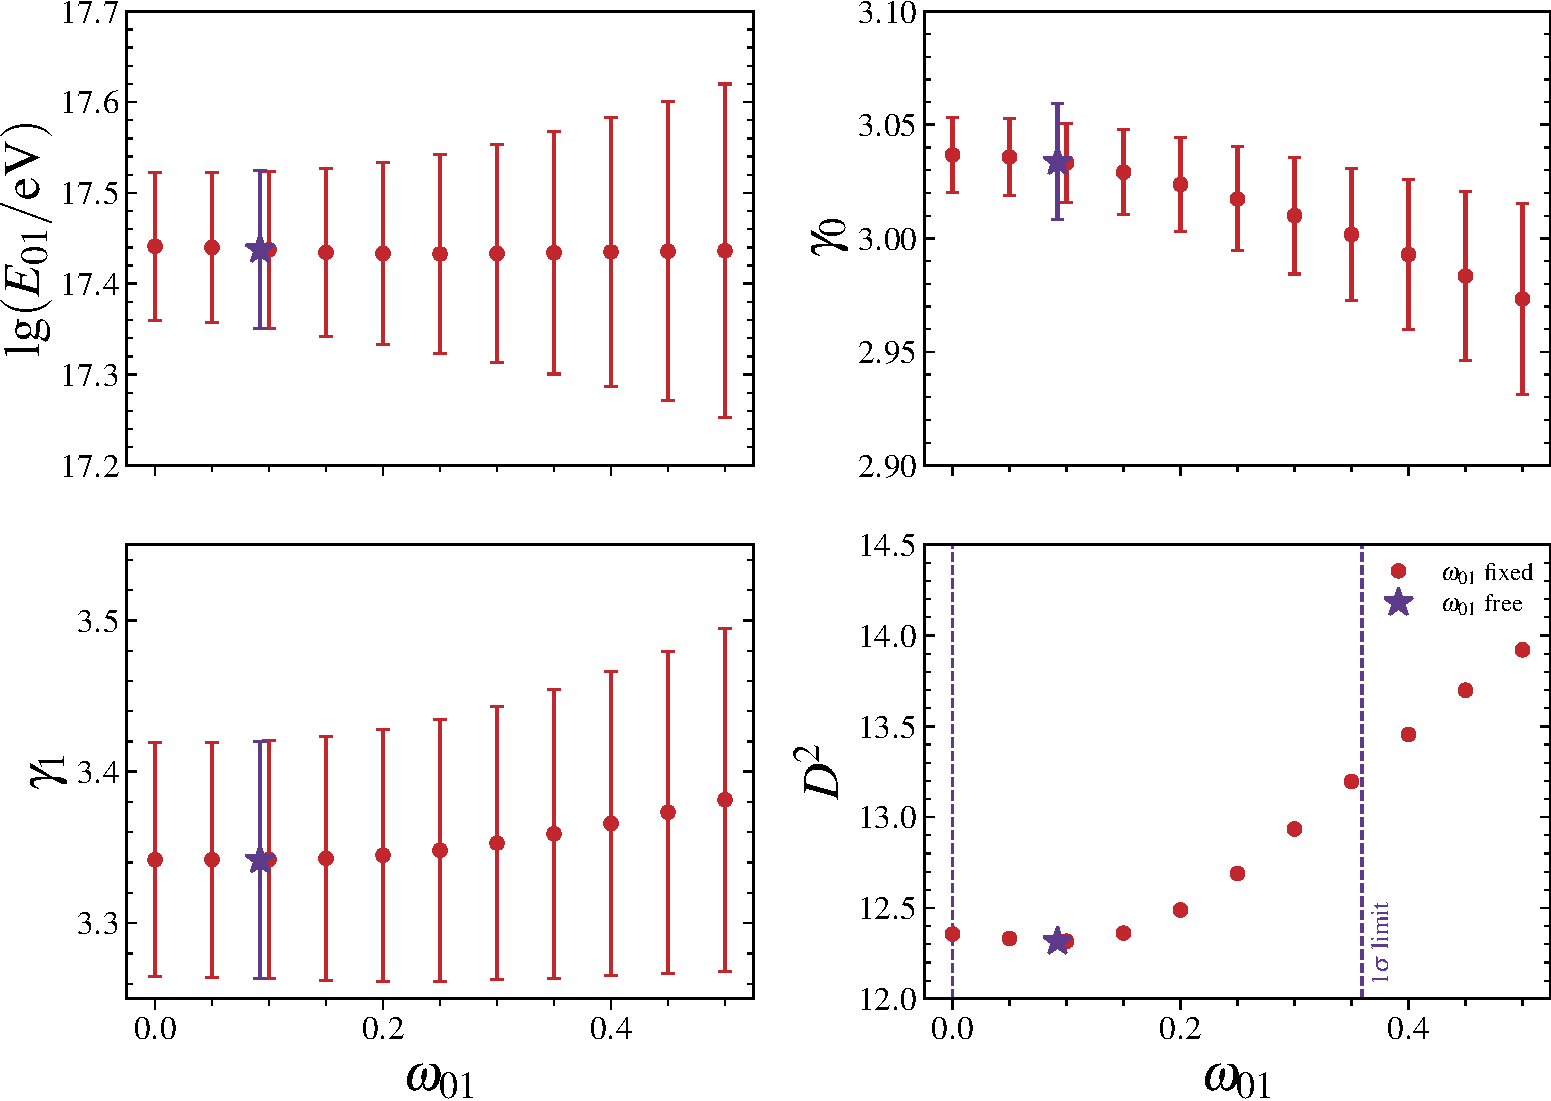
\includegraphics[width=\linewidth]{figures/chapter_spectrum/omega_dependence_2x2.pdf}
    \caption{
        Dependence of the fitted second-knee parameters and Poisson deviance
        on the assumed transition width $\omega_{01}$ for the \sd{433}
        spectrum. Circles show fits with $\omega_{01}$ fixed, including
        the sharp broken-power-law limit at $\omega_{01}=0$, while the star
        indicates the result obtained when $\omega_{01}$ is left free.
        The error bars represent the statistical uncertainties of the fits.
        The dashed vertical lines in the lower-right panel indicate the
        $1\sigma$ limits of the free-$\omega_{01}$ fit.
    }
    \label{fig:omega_study}
\end{figure}

The toy Monte-Carlo studies and the profile-likelihood scan of the measured data lead to consistent conclusions.
The closure test shows that fixing $\omega_{01}=0.05$ does not introduce a significant bias in the reconstructed second-knee energy or spectral indices, even when the injected transition is substantially broader.
Similarly, the scan of the measured data shows that the variations induced by the assumed transition width remain within the statistical uncertainties.
No additional systematic uncertainty is therefore assigned to the choice of $\omega_{01}$.

A summary of the contributions to the systematic uncertainties of the fitted spectral parameters is presented in \cref{table:sd433_parameter_systematics}.
The FD energy scale dominates the uncertainties in the normalization and second-knee energy, while the calibration parameters provide the largest contribution to the uncertainties in the spectral indices.
The detector-response uncertainties are subdominant throughout the measured energy range.
The exposure uncertainty affects only the normalization.
Since the different sources are treated as uncorrelated, the total systematic uncertainty for each parameter is obtained by adding the individual contributions in quadrature.

\begin{table}
    \centering
    \caption{
        Contributions to the systematic uncertainties of the fitted \sd{433} spectral parameters.
        The values correspond to the largest absolute variation obtained for each source.
        The uncertainty in $J_0$ is expressed in units of
        $10^{-13}\,\mathrm{km^{-2}\,yr^{-1}\,sr^{-1}\,eV^{-1}}$.
        The total is obtained by adding the independent contributions in quadrature.
    }
    \label{table:sd433_parameter_systematics}
    \begin{tabular}{lcccc}
        \hline
        Source
        & $\Delta J_0$
        & $\Delta\lg(E_{01}/\mathrm{eV})$
        & $\Delta\gamma_0$
        & $\Delta\gamma_1$ \\
        \hline
        FD energy scale
        & $0.277$ & $0.100$ & $0.024$ & $0.055$ \\
        Calibration
        & $0.156$ & $0.024$ & $0.083$ & $0.095$ \\
        Energy resolution
        & $0.008$ & $0.003$ & $0.005$ & $0.002$ \\
        Composition: bias
        & $0.038$ & $0.006$ & $0.026$ & $0.019$ \\
        Composition: efficiency
        & $0.005$ & $0.032$ & $0.019$ & $0.011$ \\
        Exposure
        & $0.028$ & $0$ & $0$ & $0$ \\
        Transition width
        & $0$ & $0$ & $0$ & $0$ \\
        \hline
        \textbf{Total}
        & $\mathbf{0.321}$
        & $\mathbf{0.108}$
        & $\mathbf{0.092}$
        & $\mathbf{0.112}$ \\
        \hline
    \end{tabular}
\end{table}

\begin{table}
    \centering
    \caption{
        Best-fit values of the \sd{433} spectral parameters.
        The first uncertainty is statistical and the second systematic.
        The transition width is fixed in the fit.
    }
    \label{table:sd433_spectral_parameters}
    \begin{tabular}{lc}
        \hline
        Parameter & Value $\pm\sigma_{\mathrm{stat}}\pm\sigma_{\mathrm{syst}}$ \\
        \hline
        $J_0/
        \left(
        \mathrm{km^{-2}\,yr^{-1}\,sr^{-1}\,eV^{-1}}
        \right)$
        & $(0.9125\pm0.0054\pm0.321)\times10^{-13}$ \\
        $\gamma_0$
        & $3.036\pm0.017\pm0.092$ \\
        $E_{01}/\mathrm{eV}$
        & $(2.75\pm0.52\pm0.68)\times10^{17}$ \\
        $\gamma_1$
        & $3.342\pm0.078\pm0.112$ \\
        $\omega_{01}$
        & $0.05$ -- fixed \\
        \hline
    \end{tabular}
\end{table}

\section{Summary of the chapter}

This chapter presents the measurement of the cosmic-ray energy spectrum with the \sd{433} array using data reconstructed from the previous chapter and recorded between July 2018 and December 2021.
The raw flux was obtained from the observed event counts and the geometrical exposure determined in \cref{chap:sd433_dataset}.

To remove detector effects in the spectrum measurement, a forward-folding procedure was developed to be included in the spectrum fit.
The detector response was incorporated into a migration matrix describing the probability that an event with true energy in bin $j$ is reconstructed in bin $i$.
The matrix accounts for the energy-dependent detection efficiency, bias, and finite resolution of the \sd{433}.
Although its exact definition depends on the assumed spectral model, this dependence can be neglected when the true-energy binning is sufficiently fine.
A true-energy bin width of $\Delta\lg(E_j/\mathrm{eV})=0.01$ was therefore adopted, compared with $\Delta\lg(E_i/\mathrm{eV})=0.1$ in reconstructed energy.

This approximation was benchmarked before it was applied to the measured spectrum.
The expected reconstructed event counts obtained with the approximate matrix were compared with those calculated using the exact, spectrum-dependent expression for an injected power-law spectrum.
The relative differences were found to be negligible across the full energy range.
This validation showed that the approximate matrix preserves the detector response while avoiding the need to assume a the spectral parameters a priori or recalculate the matrix at every step of the fit.

The validated migration matrix was subsequently used in a forward-folding Poisson-likelihood fit.
Once the best-fit spectral parameters were obtained, the ratio between the expected true and reconstructed event counts provided the correction factors used to unfold the measured flux.

A simple power law is rejected with a $p$-value of
\SDFourThreeThreePowerLawPValue, providing evidence for a change in the spectral slope.
The spectrum is therefore described using a broken power law with a smooth transition.
The fit yields a second-knee energy of
$E_{01}=(2.75\pm0.52\pm0.68)\times10^{17}\,\mathrm{eV}$,
with spectral indices
$\gamma_0=3.036\pm0.017\pm0.092$ and
$\gamma_1=3.342\pm0.078\pm0.112$
below and above the feature, respectively.
The complete set of fitted parameters is summarized in
\cref{table:sd433_spectral_parameters}.

Toy Monte-Carlo studies show that the available \sd{433} statistics are insufficient to constrain the transition width.
It is therefore fixed to $\omega_{01}=0.05$, following the value adopted by the Pierre Auger Observatory for spectral features whose transition widths could not be constrained.
The toy studies and the scan of the measured data show that this choice does not introduce a significant bias in the reconstructed second-knee energy or spectral indices.

The systematic study identifies the inherited \gls{fd} energy-scale uncertainty as the dominant contribution to the flux normalization and the position of the Second Knee.
The systematic uncertainty in the \sd{433} energy calibration parameters produces the next-largest contribution and has the strongest effect on the spectral indices, while uncertainties associated with the detector response are smaller.
The measurement therefore establishes the spectral steepening in the energy range covered by the \sd{433} and places it within the current statistical and systematic uncertainties.
The transition width will be investigated with greater sensitivity using the combined \sd{433} and \sd{750} spectrum.

\end{document}
